%%% Local Variables:
%%% mode: latex
%%% TeX-master: t
%%% End:
\documentclass{beamer}
\usepackage[utf8]{inputenc}
\usepackage[german]{babel}
\usepackage{graphics}
\usepackage{listings}
\usepackage{caption}

\captionsetup{font=scriptsize,labelfont=scriptsize}

\usetheme{default}
\usecolortheme{rose}

\DeclareGraphicsRule{.pdftex}{pdf}{.pdftex}{}

% \lstdefinelanguage{cfengine}
%   {morekeywords={import,classes,control,admit,copy,editfiles,processes,shellcommands},
%    sensitive=false,
%    morecommment[l]{//},
%   }

\newcommand\Fontvi{\fontsize{6}{7.2}\selectfont}

\lstset{
basicstyle=\tiny,
stringstyle=\tiny,
numbers=left,
numberstyle=\tiny,
stepnumber=2,
frame=single,
%language=cfengine,
captionpos=b
}

\title{System Automation mit Puppet und Foreman\\}
\author{Toni Schmidbauer}

\begin{document}

\begin{frame}
\center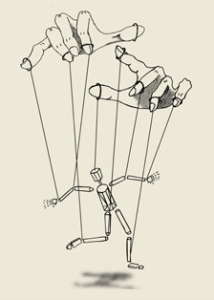
\includegraphics[height=2.5cm,width=2cm]{../pics/puppet.png}
\titlepage

\end{frame}

\begin{frame}
  \frametitle{whoami}
  \begin{itemize}
  \item SysAdmin@s-itsolutions
  \item toni@stderr.at
  \item http://github.com/tosmi
  \item stderr@jabber.org
  \end{itemize}
\end{frame}
\begin{frame}

  \frametitle{Agenda}

  \begin{itemize}
  \item Kurze Umfrage
  \item Was ist Puppet?
  \item Was ist Foreman?
  \item Puppet@s-iTSolutions
  \item Modul Entwicklung
  \item Deployment Prozess
  \end{itemize}

\end{frame}

\begin{frame}
\center{\huge{Umfrage}}
\end{frame}

\begin{frame}[fragile]
  \frametitle{Was ist Puppet?}

  \begin{lstlisting}
    class mypuppetconfig {

      user { 'linuxwochen':
        ensure => present,
        uid => 4711,
        gid => 4711,
      }

      package { 'emacs':
        ensure => installed
      } ->
      package { 'vi':
        ensure => absent,
      }
    }
  \end{lstlisting}
\end{frame}

\begin{frame}[fragile]
  \frametitle{Zuordnung von Klassen}

  \begin{lstlisting}
    node linuxwochen {
      include mypuppetconfig
    }
  \end{lstlisting}

  \begin{itemize}
  \item oder über einen External Node Classifier (Foreman)
  \end{itemize}
\end{frame}

\begin{frame}
  \frametitle{Was ist Foreman?}
  \begin{figure}[ht]
    \centering
    \framebox{
      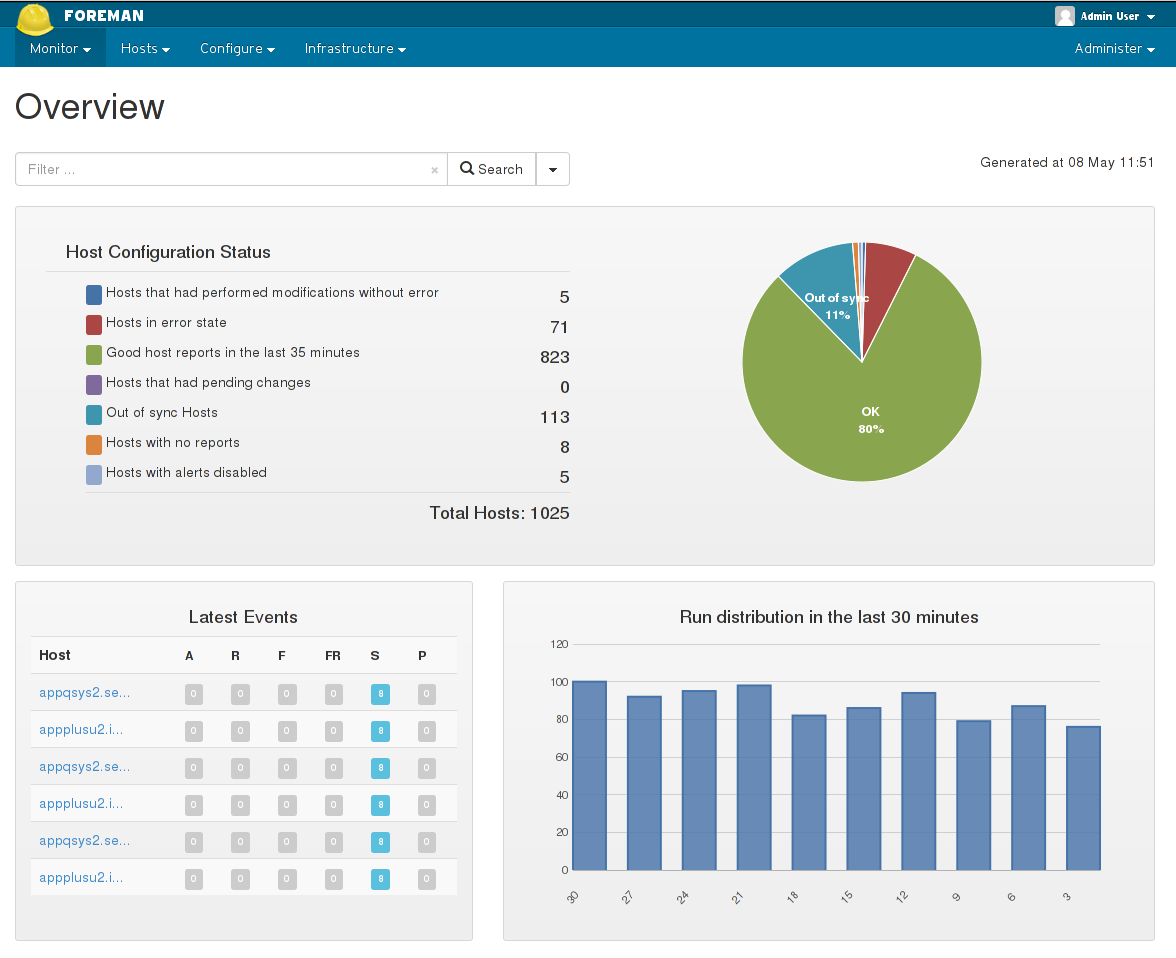
\includegraphics[height=7.5cm,width=10cm]{../pics/foreman_dashboard.png}
    }
    \label{fig:stack}
  \end{figure}
\end{frame}

\begin{frame}
  \frametitle{Und jetzt?}

  \begin{itemize}
  \item Wie verwaltet wir unseren Puppet Code?cm
  \item Wie organisieren wir Module?
  \item Wie soll eine Entwicklungsumgebung aussehen?
  \item Ein Repository für alle Module?
  \item Pro Modul ein Repository?
  \item Wie verwalten wir Module von PuppetForge?
  \item Wie erfolgt das Deployment des Codes?
  \item Was ist mit Unittests?
  \end{itemize}
\end{frame}


\end{document}